\section{Experimentos y análisis de resultados}
	
	\subsection{Procedimiento de desarrollo de la práctica}
	
	\paragraph{}Para realizar la práctica, se ha optado por implementar las heurísticas propuestas en el lenguaje de programación \textsc{Java}. El ejecutable que se entrega junto a este documento ha sido compilado bajo \textsc{ Apache NetBeansIDE 12.0}.
	
	\subsubsection{Equipo de pruebas}
	
	\paragraph{}Los resultados de las heurísticas han sido obtenidos en el siguiente equipo:
	
		\begin{itemize}
			
			\item Host: 80WK Lenovo Y520-15IKBN
			\item S.O: KDE neon User Edition 5.20 x86 64
			\item Kernel: 5.4.0-52-generic
			\item CPU: Intel i5-7300HQ (4) @ 3.500GHz
			\item GPU: NVIDIA GeForce GTX 1050 Mobile
			\item GPU: Intel HD Graphics 630
			\item Memoria RAM : 7837 MiB.
			
		\end{itemize}

	\subsubsection{Manual de usuario}
	
		\paragraph{}Para ejecutar el software asegúrese de que el archivo .jar proporcionado se ubica en el mismo directorio que la carpeta \emph{archivos}. 
		
		\paragraph{}Cuando se muestre la GUI, podrá seleccionar la heurística que desee mediante el botón correspondiente. Una vez empiece la ejecución de una heurística no sera posible seleccionar otra hasta que finalice su ejecución. Los resultados finales se mostrarán en el cuadro de texto, a su vez, se generan los log correspondientes a cada archivo y semilla en la carpeta Log.
	
		\begin{figure}[H]
		
			\centering
			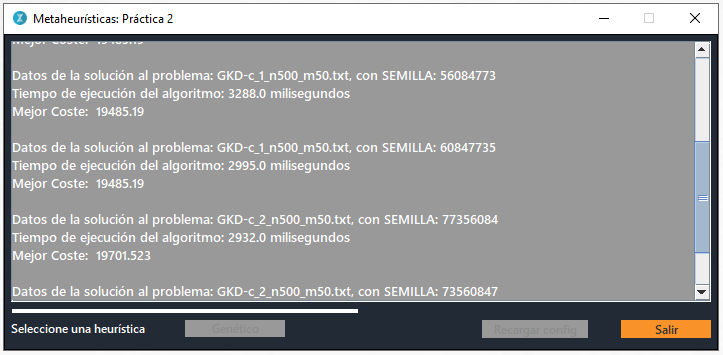
\includegraphics[scale=0.4]{img/GUI}
			\caption{GUI}
		
		\end{figure}
	
	\subsection{Parámetros de los algoritmos}
	
		\subsubsection{Genético}
		\paragraph{}Para regular el comportamiento de los algoritmos genéticos, se han definido los siguientes parámetros en el archivo de configuración:ç
		
		\begin{itemize}
			
			\item Semilla: Número utilizado para la generación de números pseudoaleatorios, valor por defecto : 77356084
			\item Evaluaciones:  Número máximo de evaluaciones, valor por defecto: 50000
			\item Elitismo: Número máximo de los mejores individuos de la generación anterior que pasan a la siguiente.
			\item OperadorMPX: Booleano que indica si se debe usar el operador de cruce MPX (true), o el cruce en dos puntos (false).
			\item Probabilidad de mutacion: Probabilidad de mutación que se aplica a cada gen, valor por defecto: 0,01.
			\item Probabilidad de reproduccion: Probabilidad de que dos individuos de la población se crucen, valor por defecto: 0,90.
			\item Cromosomas: Tamaño de la población, valor por defecto: 50.
			\item Probabilidad MPX: Determina la cantidad de genes que se heredan del primer padre, para el operador de cruce MPX, valor por defecto: 0,50.
			
		\end{itemize}

	
	\subsubsection{Semillas}
	
	\paragraph{}Para la generación de números pseudoaleatorios se utiliza una semilla previamente definida en el archivo de configuración, en este caso es 77356084. Esta semilla se va rotando en las 5 iteraciones de cada archivo.
	
	
	\paragraph{} 77356084 $\rightarrow$ 73560847 $\rightarrow$ 35608477  ...
	
	
	\subsection{Análisis de los resultados}
	
	\subsubsection{Efectos de la mutación}
	
	\paragraph{} La mutación en los algoritmos genéticos es una técnica de diversificación/exploración, la cual puede ayudar a salir de óptimos locales, no obstante, su porcentaje de aplicación debe ser reducido. Esto es debido a que una alta probabilidad de mutación puede alterar considerablemente las soluciones obtenidas, resultando en una calidad inferior de las mismas.
	
	Para reflejar este comportamiento de la mutación, se ha seleccionado el conjunto de datos SOM, y se ha establecido 3 valores distintos de probabilidad de mutación: 0,01, 0,05 y 0,09. Cada Probabilidad de mutación se ha aplicado en 5 iteraciones, con distinta semilla para cada archivo. Posteriormente se ha obtenido la media de las 5 iteraciones para cada archivo y probabilidad de mutación, de dichos resultados se ha obtenido la siguiente gráfica:
	
	\begin{figure}[H]
		
		\centering
		\includegraphics[scale=0.8]{img/Mutación}
		\caption{Diferencias en porcentajes respecto a los óptimos globales}
		
	\end{figure}
	
	\paragraph{}Como se puede observar, un mayor porcentaje de mutación, empeora los resultados obtenidos mediante algoritmos genéticos.
	
	\begin{figure}[H]
		
		\centering
		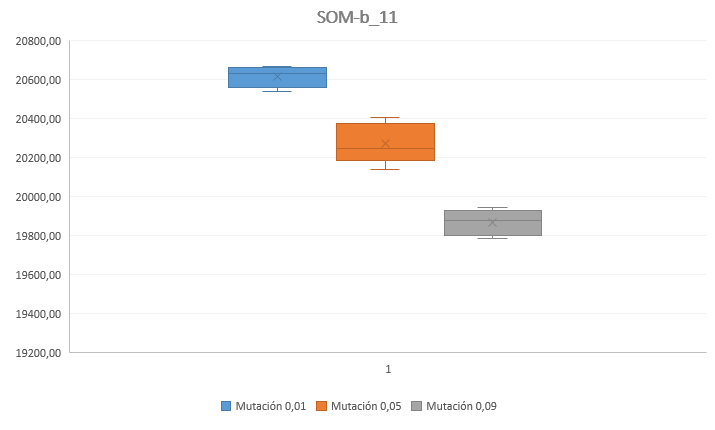
\includegraphics[scale=0.7]{img/BigotesMutacionSOM_11}
		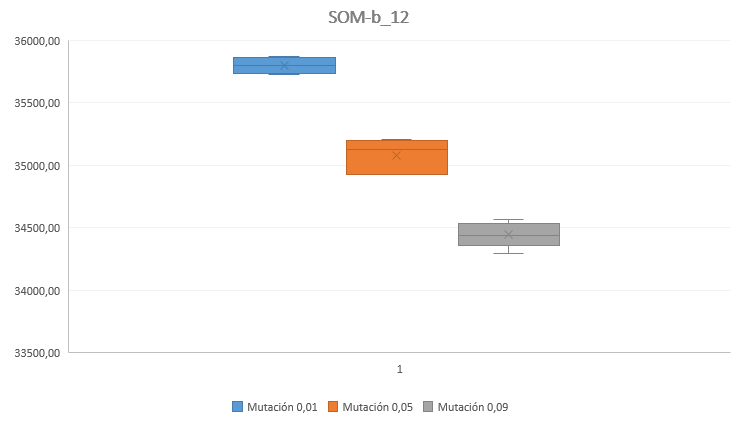
\includegraphics[scale=0.7]{img/BigotesMutacionSOM_12}
		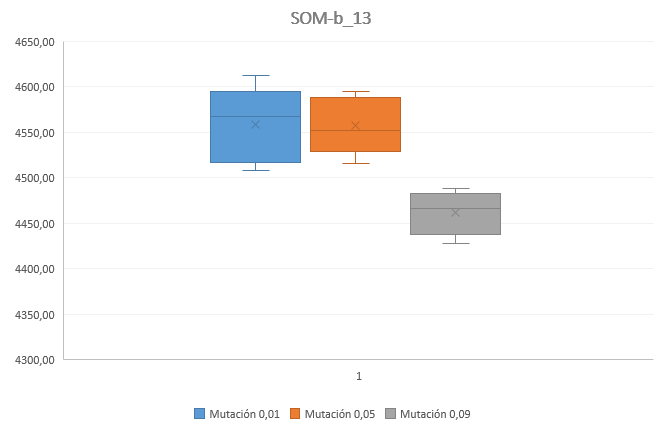
\includegraphics[scale=0.7]{img/BigotesMutacionSOM_13}
		
	\end{figure}
	
	\paragraph{}A raíz de los resultados obtenidos anteriormente, se reflexionó sobre el impacto que tendría fijar una capacidad de mutación nula. Al realizar las pruebas, se obtuvo que fijar una mutación al 0,00 elimina parte de la capacidad de mejora, siendo sus resultados inferiores a una mutación del 0,01. Esto es debido a que el comportamiento del algoritmo sin la mutación se basa en la explotación.
	
	\begin{figure}[H]
		
		\centering
		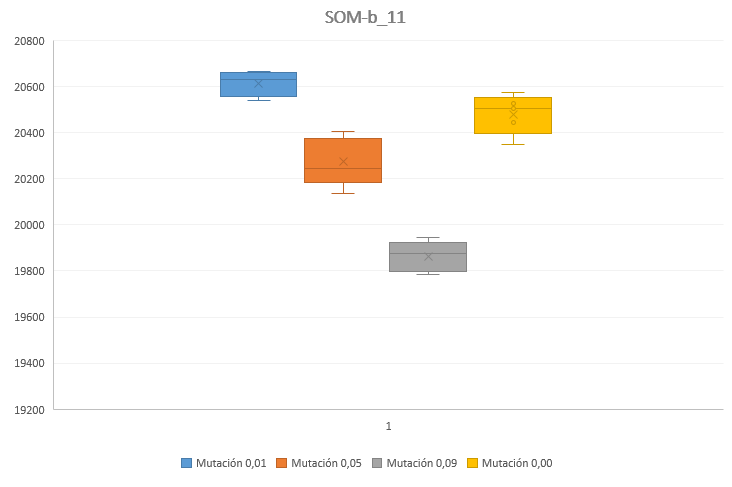
\includegraphics[scale=0.7]{img/BigotesMutacion0_SOM_1}
	\end{figure}
	\begin{figure}[H]
		
		\centering
		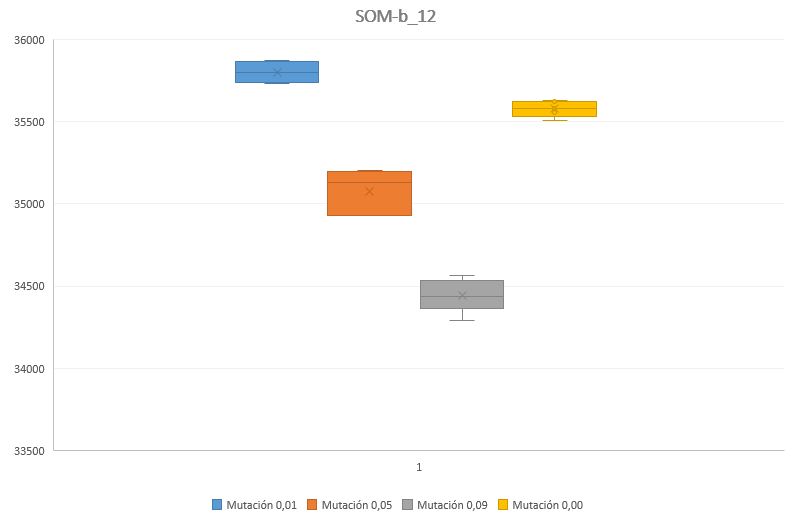
\includegraphics[scale=0.7]{img/BigotesMutacion0_SOM_2}
		
	\end{figure}
	\begin{figure}[H]
		
		\centering
		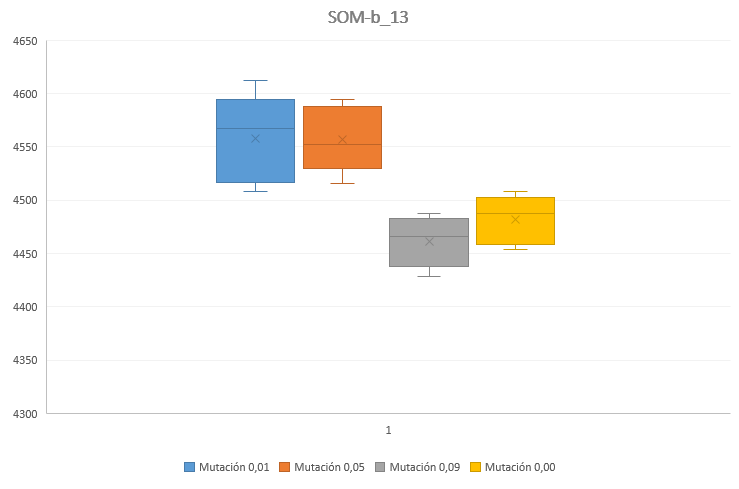
\includegraphics[scale=0.7]{img/BigotesMutacion0SOM_3}
		
	\end{figure}

	\subsubsection{Resultados obtenidos durante la experimentación}

	\paragraph{} En las gráficas siguientes se muestra la evolución del mejor coste encontrado hasta el momento en la ejecución de cada uno de los algoritmos conforme aumenta el número de evaluaciones realizadas para cada uno de los problemas. La semilla utilizada ha sido 35608477.

	\begin{figure}[H]
		\centering
		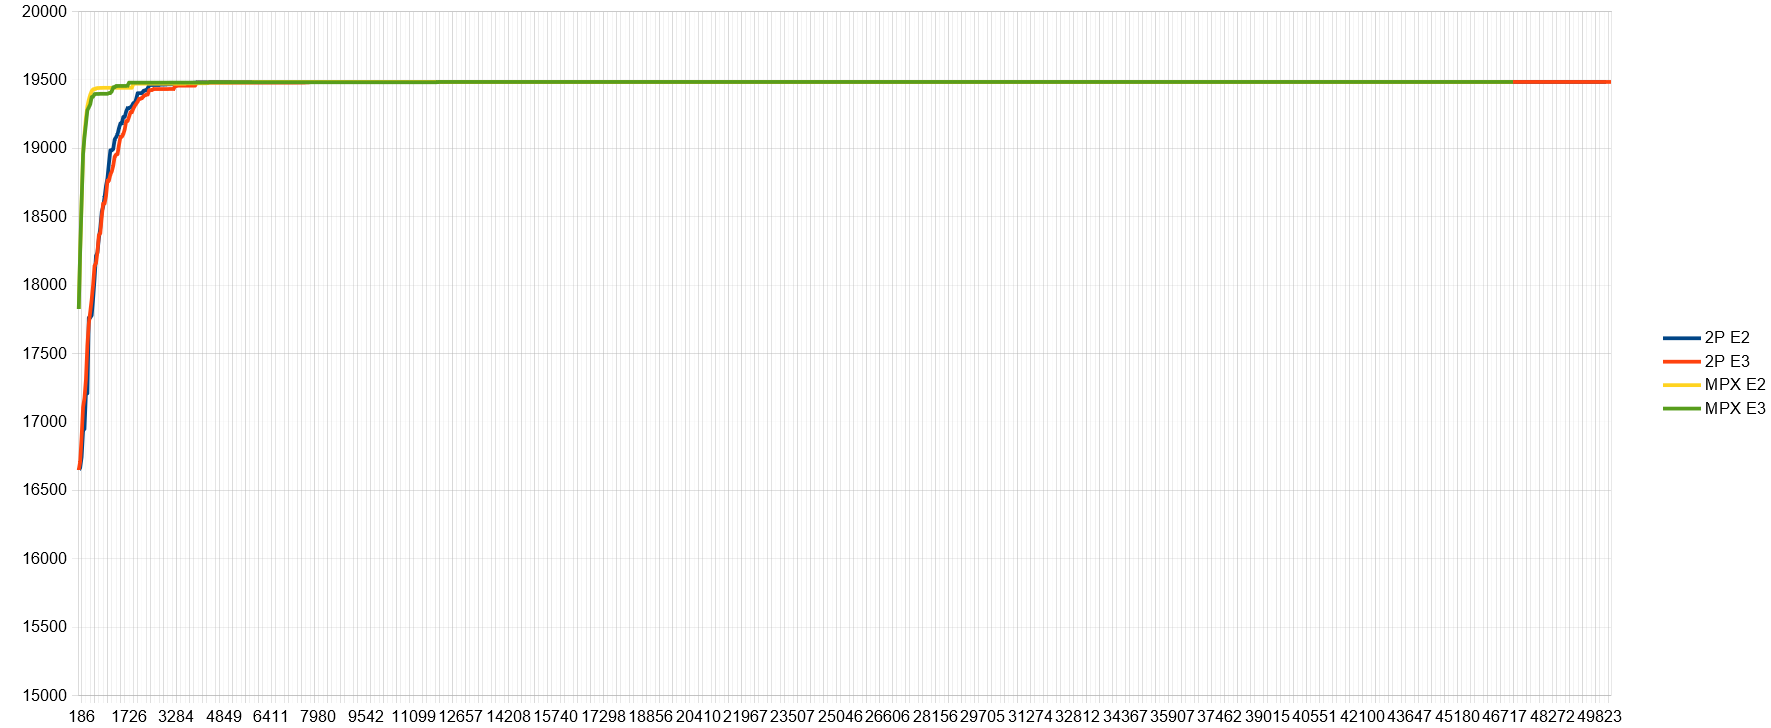
\includegraphics[scale=0.3]{img/35608477_GKD-c_1_n500_m50.png}
		\caption{Evolución del mejor coste en la ejecución de todos los algoritmos respecto al número de evaluaciones para el problema GKD-c1, semilla 35608477}
		\label{gkd-c1_historico}
	\end{figure}

	\paragraph{}Para el problema GKD-c1 los algoritmos MPX empiezan a encontrar soluciones aceptables en torno a las 100 evaluaciones realizadas para los dos elitismos. Los algoritmos de cruce en dos puntos empiezan a obtener soluciones aceptables a partir de las 420 evaluaciones para una élite = 2, y a partir de las 372 evaluaciones para una élite = 3. Hemos considerado una solución aceptable aquella solución que difiere como máximo un 10\% respecto al óptimo global. En este problema las soluciones óptimas son todas aquellas cuyo coste es superior a 17.536,669.
	
	\paragraph{}En la ejecución del algoritmo MPX con un elitismo = 2, el mejor coste obtenido se estabiliza en 19.485,19 a partir de las 6.250 evaluaciones, permaneciendo inalterable hasta finalizar las 50.000 evaluaciones objetivo.
	
	\paragraph{}En la ejecución del algoritmo MPX con un elitismo = 3, el mejor coste obtenido se estabiliza en 19.485,19 a partir de las 12.700 evaluaciones, permaneciendo inalterable hasta alcanzar las 50.000 evaluaciones objetivo.
	
	\paragraph{}En la ejecución del algoritmo de corte en dos puntos con un elitismo = 2, el mejor coste obtenido se estabiliza en 19.485,19 a partir de las 4.419 evaluaciones, permaneciendo estable hasta finalizar las 50.000 evaluaciones objetivo.
	
	\paragraph{}En la ejecución del algoritmo de corte en dos puntos con un elitismo = 3, el mejor coste obtenido se estabiliza en 19.485,19 a partir de las 8.452 evaluaciones, permaneciendo inalterable hasta alcanzar las 50.000 evaluaciones objetivo.
	
	\paragraph{}En todos los algoritmos ejecutados obtenemos un coste final = 19.485,19, coincidiendo con el óptimo global.

	\begin{figure}[H]
		\centering
		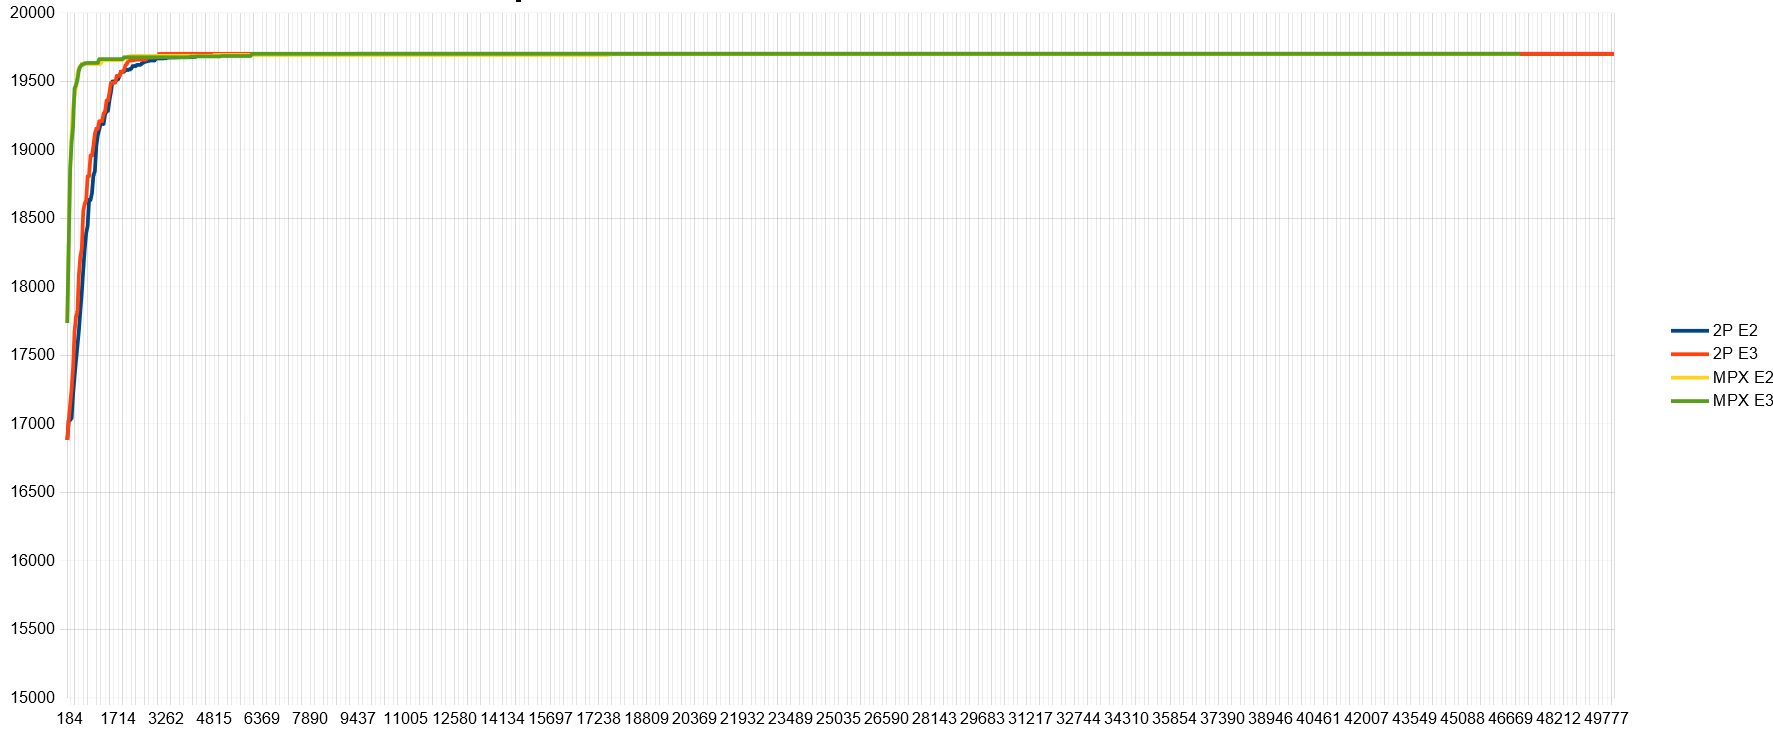
\includegraphics[scale=0.3]{img/35608477_GKD-c_2_n500_m50.png}
		\caption{Evolución del mejor coste en la ejecución de todos los algoritmos respecto al número de evaluaciones para el problema GKD-c2, semilla 35608477}
		\label{gkd-c2_historico}
	\end{figure}

	\paragraph{}Para el problema GKD-c2 los algoritmos MPX empiezan a encontrar soluciones aceptables en torno a las 100 evaluaciones realizadas para los dos elitismos. Los algoritmos de cruce en dos puntos empiezan a obtener soluciones aceptables a partir de las 321 evaluaciones para una élite = 2, y a partir de las 277 evaluaciones para una élite = 3. En este problema las soluciones óptimas son todas aquellas cuyo coste es superior a 17.731,383.
	
	\paragraph{}En la ejecución del algoritmo MPX con un elitismo = 2, el mejor coste obtenido se estabiliza en 19.700,34 a partir de las 18.800 evaluaciones, permaneciendo inalterable hasta finalizar las 50.000 evaluaciones objetivo.
	
	\paragraph{}En la ejecución del algoritmo MPX con un elitismo = 3, el mejor coste obtenido se estabiliza en 19.701,523 a partir de las 6.600 evaluaciones, permaneciendo inalterable hasta alcanzar las 50.000 evaluaciones objetivo.
	
	\paragraph{}En la ejecución del algoritmo de corte en dos puntos con un elitismo = 2, el mejor coste obtenido se estabiliza en 19.701,523 a partir de las 9.396 evaluaciones, permaneciendo estable hasta finalizar las 50.000 evaluaciones objetivo.
	
	\paragraph{}En la ejecución del algoritmo de corte en dos puntos con un elitismo = 3, el mejor coste obtenido se estabiliza en 19.701,523 a partir de las 4.108 evaluaciones, permaneciendo inalterable hasta alcanzar las 50.000 evaluaciones objetivo.
	
	\paragraph{}En todos los algoritmos ejecutados, menos en el MPX con elitismo = 2, obtenemos un coste final = 19.701,523 , difiriendo en un 0,0000008\% aproximadamente respecto al óptimo global = 19.701,537.
	
	\paragraph{}En el caso del algoritmo MPX con elitismo = 3, obtenemos un coste final = 19.700,34. Este coste difiere un 0,00007\% del óptimo global.

	\begin{figure}[H]
		\centering
		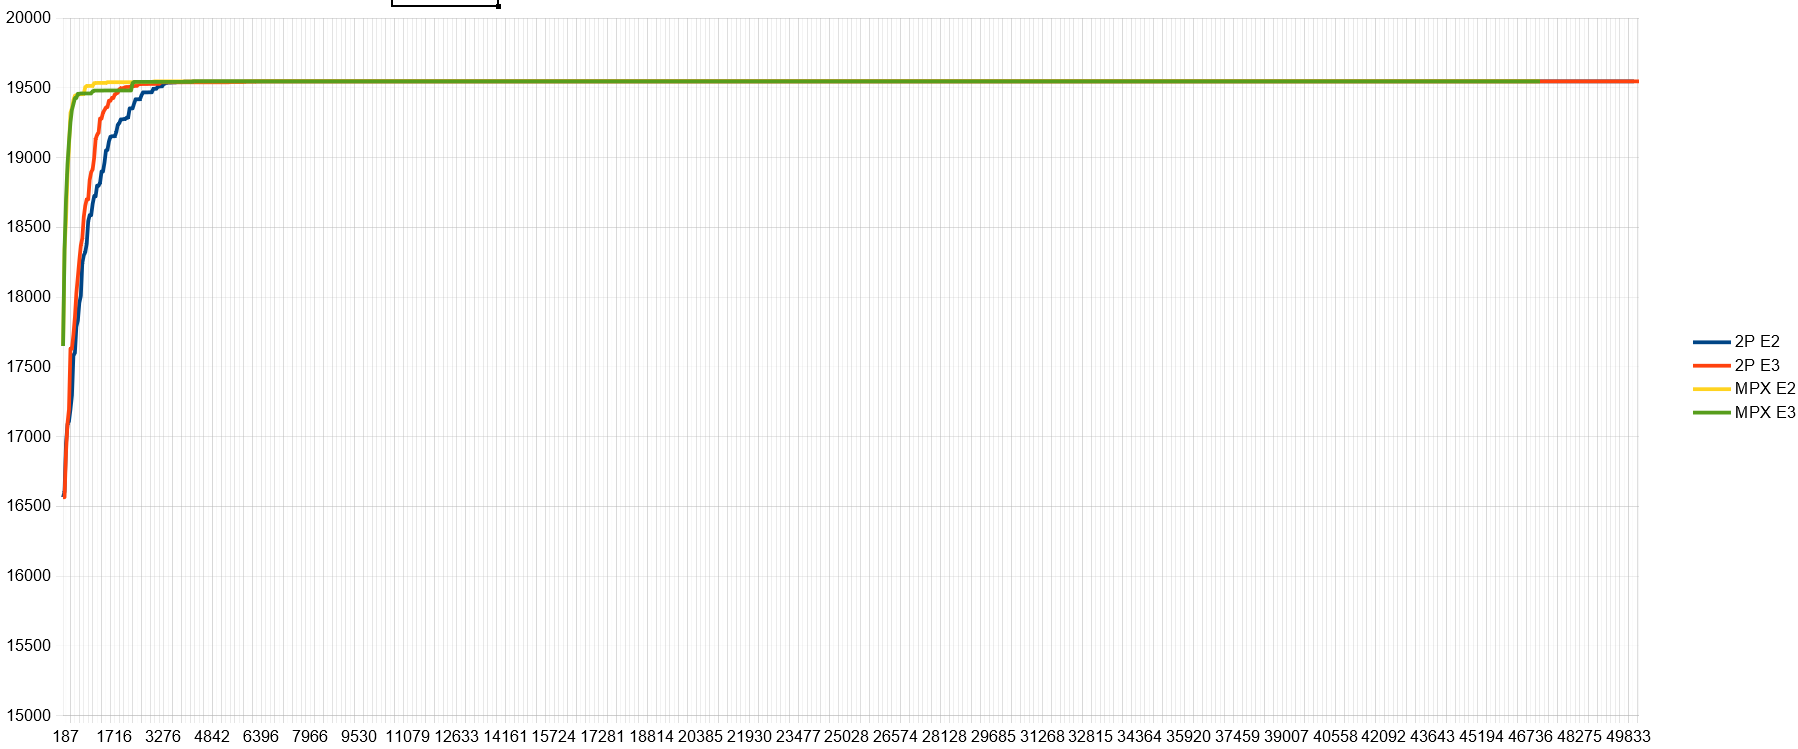
\includegraphics[scale=0.3]{img/35608477_GKD-c_3_n500_m50.png}
		\caption{Evolución del mejor coste en la ejecución de todos los algoritmos respecto al número de evaluaciones para el problema GKD-c3, semilla 35608477}
		\label{gkd-c3_historico}
	\end{figure}

	\paragraph{}Para el problema GKD-c3 los algoritmos MPX empiezan a encontrar soluciones aceptables en torno a las 100 evaluaciones realizadas para los dos elitismos. Los algoritmos de cruce en dos puntos empiezan a obtener soluciones aceptables a partir de las 467 evaluaciones para una élite = 2, y a partir de las 324 evaluaciones para una élite = 3. En este problema las soluciones óptimas son todas aquellas cuyo coste es superior a 17.592,486.
	
	\paragraph{}En la ejecución del algoritmo MPX con un elitismo = 2, el mejor coste obtenido se estabiliza en 19.547,215 a partir de las 3.200 evaluaciones, permaneciendo inalterable hasta finalizar las 50.000 evaluaciones objetivo.
	
	\paragraph{}En la ejecución del algoritmo MPX con un elitismo = 3, el mejor coste obtenido se estabiliza en 19.547,215 a partir de las 4.500 evaluaciones, permaneciendo inalterable hasta alcanzar las 50.000 evaluaciones objetivo.
	
	\paragraph{}En la ejecución del algoritmo de corte en dos puntos con un elitismo = 2, el mejor coste obtenido se estabiliza en 19.547,215 a partir de las 4.459 evaluaciones, permaneciendo estable hasta finalizar las 50.000 evaluaciones objetivo.
	
	\paragraph{}En la ejecución del algoritmo de corte en dos puntos con un elitismo = 3, el mejor coste obtenido se estabiliza en 19.547,215 a partir de las 6.414 evaluaciones, permaneciendo inalterable hasta alcanzar las 50.000 evaluaciones objetivo.
	
	\paragraph{}En todos los algoritmos ejecutados obtenemos un coste final = 19.547,215, coincidiendo con el óptimo global.

	\begin{figure}[H]
		\centering
		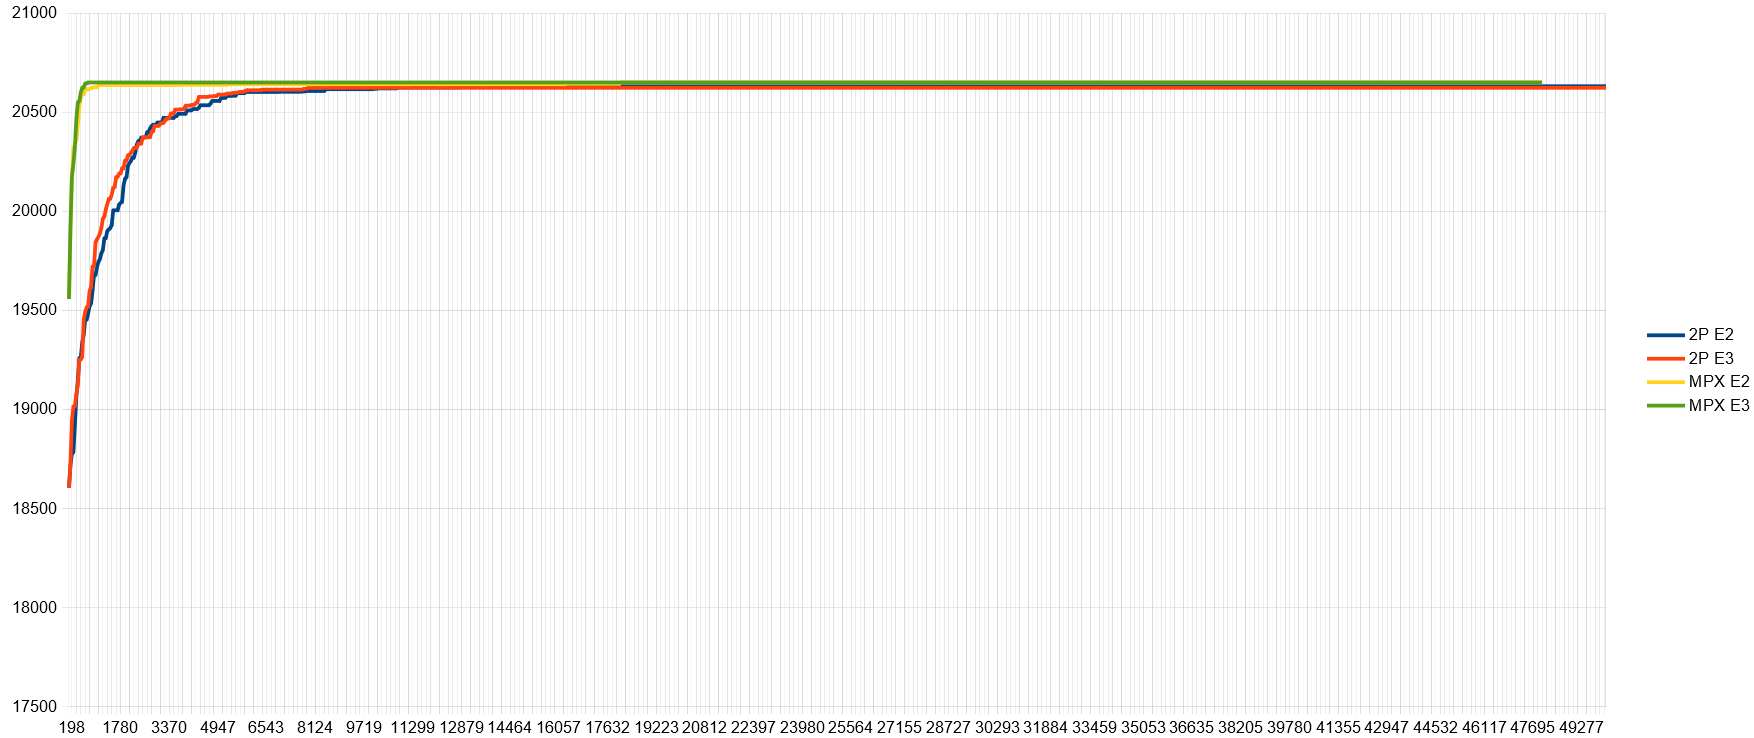
\includegraphics[scale=0.3]{img/35608477_SOM-b_11_n300_m90.png}
		\caption{Evolución del mejor coste en la ejecución de todos los algoritmos respecto al número de evaluaciones para el problema SOM-b11, semilla 35608477}
		\label{SOM-b_11_historico}
	\end{figure}

	\paragraph{}Para el problema SOM-b11 los algoritmos MPX empiezan a encontrar soluciones aceptables en torno a las 100 evaluaciones realizadas para los dos elitismos. Los algoritmos de cruce en dos puntos empiezan a obtener soluciones aceptables a partir de las 148 evaluaciones para los dos elitismos. En este problema las soluciones óptimas son todas aquellas cuyo coste es superior a 18.668,7.
	
	\paragraph{}En la ejecución del algoritmo MPX con un elitismo = 2, el mejor coste obtenido se estabiliza en 20.651 a partir de las 18.800 evaluaciones, permaneciendo inalterable hasta finalizar las 50.000 evaluaciones objetivo.
	
	\paragraph{}En la ejecución del algoritmo MPX con un elitismo = 3, el mejor coste obtenido se estabiliza en 20.650 a partir de las 750 evaluaciones, permaneciendo inalterable hasta alcanzar las 50.000 evaluaciones objetivo.
	
	\paragraph{}En la ejecución del algoritmo de corte en dos puntos con un elitismo = 2, el mejor coste obtenido se estabiliza en 20.631 a partir de las 15.280 evaluaciones, permaneciendo estable hasta finalizar las 50.000 evaluaciones objetivo.
	
	\paragraph{}En la ejecución del algoritmo de corte en dos puntos con un elitismo = 3, el mejor coste obtenido se estabiliza en 20.623 a partir de las 7.865 evaluaciones, permaneciendo inalterable hasta alcanzar las 50.000 evaluaciones objetivo.
	
	\paragraph{}En el algoritmo MPX con un elitismo = 2 obtenemos un coste final = 20.651, que difiere del óptimo global en un 0,005\% aproximadamente. El óptimo global para este problema es 20.743.
	
	\paragraph{}En el algoritmo MPX con un elitismo = 3 obtenemos un coste final = 20.650, que difiere del óptimo global en un 0,005\% aproximadamente.
	
	\paragraph{}En el algoritmo de corte en dos puntos con un elitismo = 2 obtenemos un coste final = 20.631, que difiere del óptimo global en un 0,006\% aproximadamente.
	
	\paragraph{}En el algoritmo de corte en dos puntos con un elitismo = 3 obtenemos un coste final = 20.623, que difiere del óptimo global en un 0,006\% aproximadamente.

	\begin{figure}[H]
		\centering
		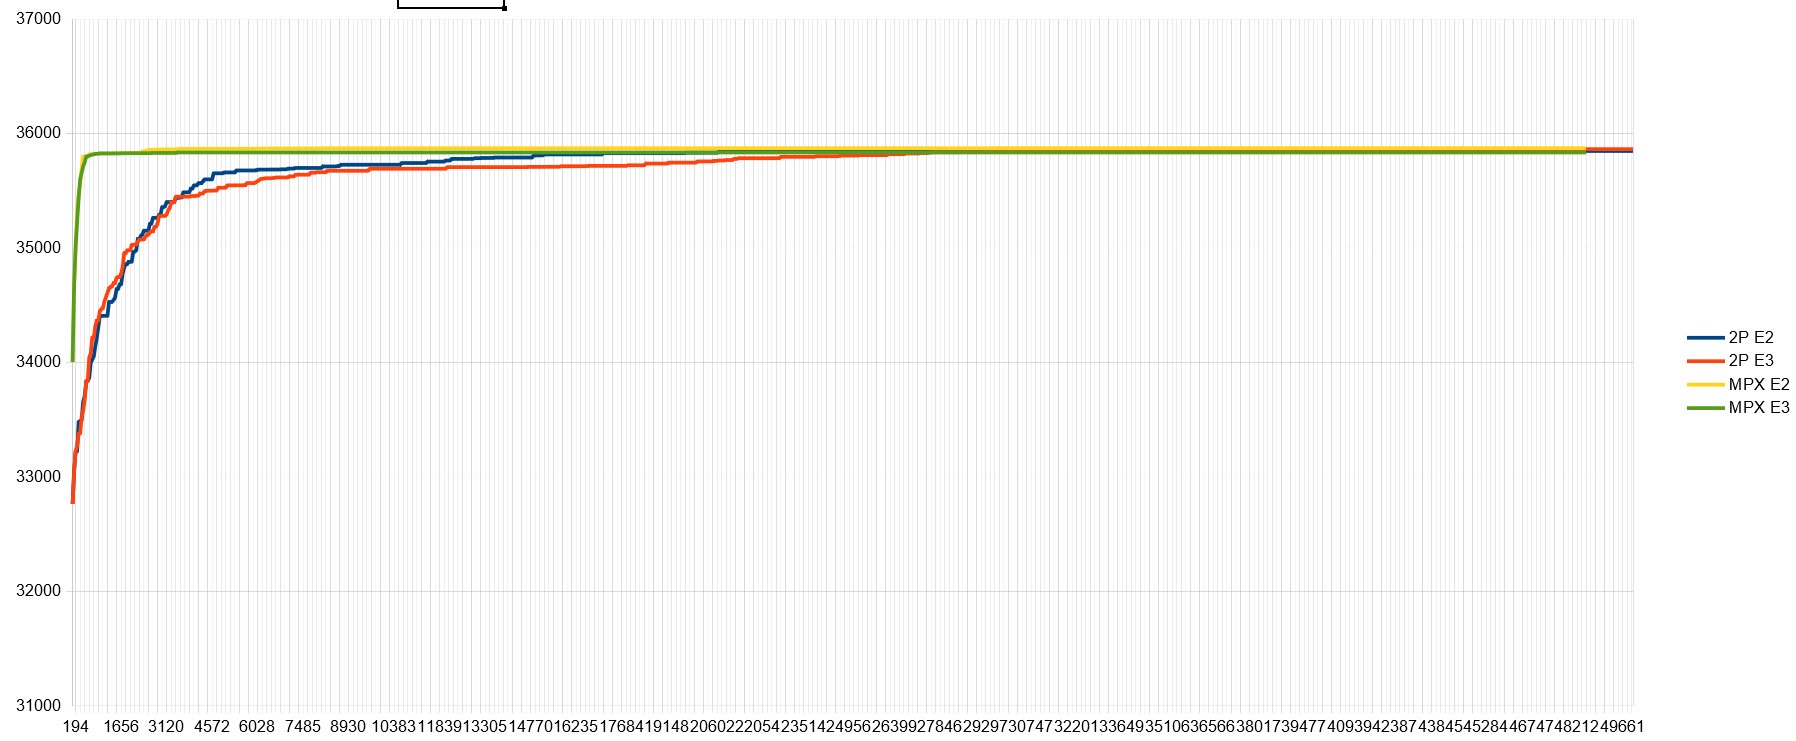
\includegraphics[scale=0.3]{img/35608477_SOM-b_12_n300_m90.png}
		\caption{Evolución del mejor coste en la ejecución de todos los algoritmos respecto al número de evaluaciones para el problema SOM-b12, semilla 35608477}
		\label{SOM-b_12_historico}
	\end{figure}

	\paragraph{}Para el problema SOM-b12 todos los algoritmos empiezan a encontrar soluciones aceptables en torno a las 100 evaluaciones realizadas para los dos elitismos. En este problema las soluciones óptimas son todas aquellas cuyo coste es superior a 32.292,9.
	
	\paragraph{}En la ejecución del algoritmo MPX con un elitismo = 2, el mejor coste obtenido se estabiliza en 35.871 a partir de las 8.400 evaluaciones, permaneciendo inalterable hasta finalizar las 50.000 evaluaciones objetivo.
	
	\paragraph{}En la ejecución del algoritmo MPX con un elitismo = 3, el mejor coste obtenido se estabiliza en 35.834 a partir de las 3.550 evaluaciones, permaneciendo inalterable hasta alcanzar las 50.000 evaluaciones objetivo.
	
	\paragraph{}En la ejecución del algoritmo de corte en dos puntos con un elitismo = 2, el mejor coste obtenido se estabiliza en 35.847 a partir de las 21.669 evaluaciones, permaneciendo estable hasta finalizar las 50.000 evaluaciones objetivo.
	
	\paragraph{}En la ejecución del algoritmo de corte en dos puntos con un elitismo = 3, el mejor coste obtenido se estabiliza en 35.863 a partir de las 39.724 evaluaciones, permaneciendo inalterable hasta alcanzar las 50.000 evaluaciones objetivo.
	
	\paragraph{}En el algoritmo MPX con un elitismo = 2 obtenemos un coste final = 35.871, que difiere del óptimo global en un 0,0003\% aproximadamente. El óptimo global para este problema es 35.881.
	
	\paragraph{}En el algoritmo MPX con un elitismo = 3 obtenemos un coste final = 35.834, que difiere del óptimo global en un 0,002\% aproximadamente.
	
	\paragraph{}En el algoritmo de corte en dos puntos con un elitismo = 2 obtenemos un coste final = 35.847, que difiere del óptimo global en un 0,001\% aproximadamente.
	
	\paragraph{}En el algoritmo de corte en dos puntos con un elitismo = 3 obtenemos un coste final = 35.863, que difiere del óptimo global en un 0,0006\% aproximadamente.

	\begin{figure}[H]
		\centering
		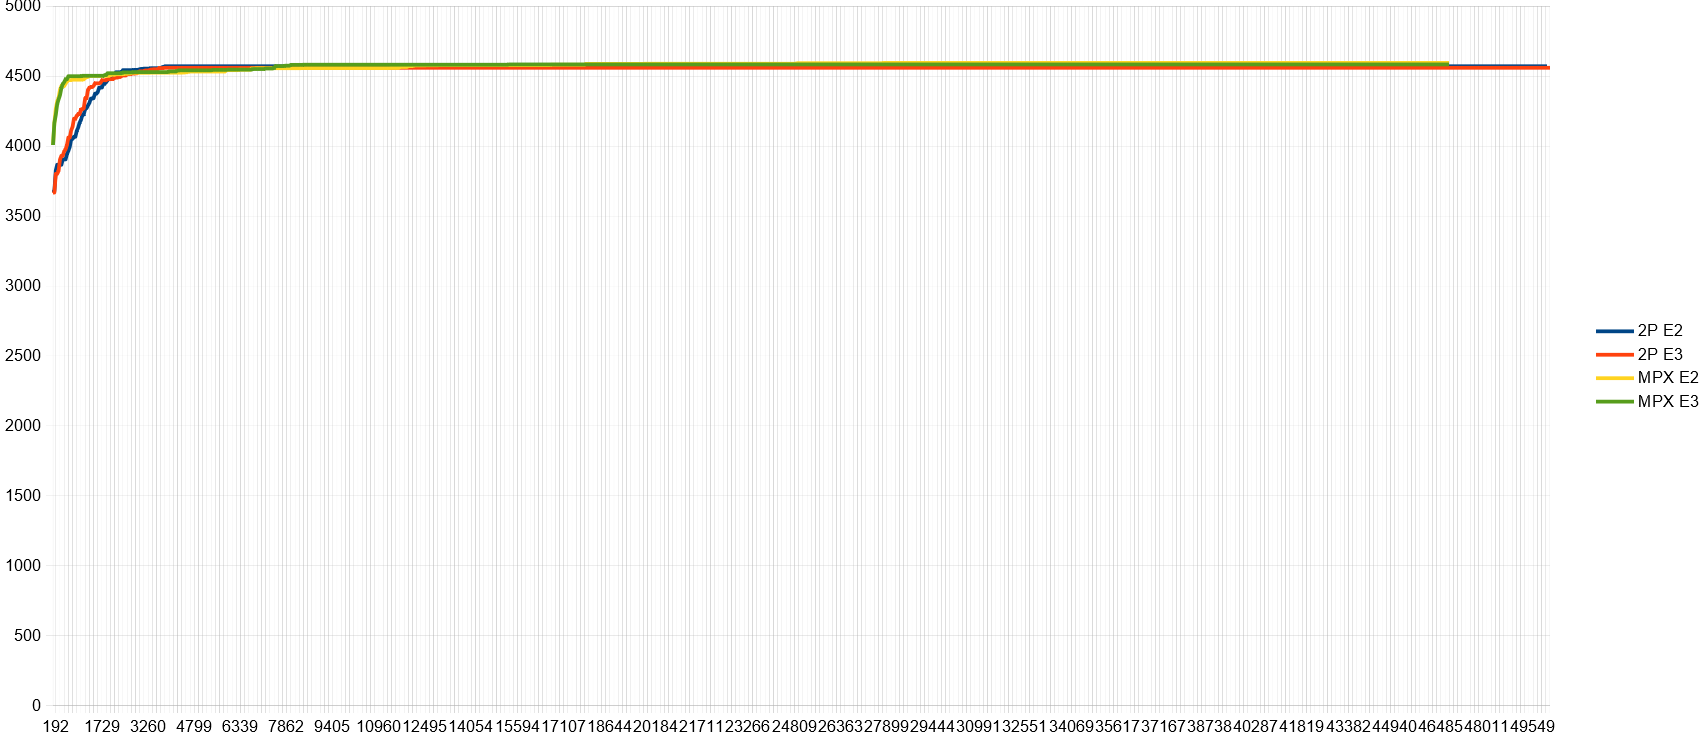
\includegraphics[scale=0.3]{img/35608477_SOM-b_13_n300_m90.png}
		\caption{Evolución del mejor coste en la ejecución de todos los algoritmos respecto al número de evaluaciones para el problema SOM-b13, semilla 35608477}
		\label{SOM-b_13_historico}
	\end{figure}

	\paragraph{}Para el problema SOM-b13 los algoritmos MPX empiezan a encontrar soluciones aceptables en torno a las 200 evaluaciones realizadas para los dos elitismos. Los algoritmos de cruce en dos puntos empiezan a obtener soluciones aceptables a partir de las 1085 evaluaciones para una élite = 2, y a partir de las 793 evaluaciones para una élite = 3. En este problema las soluciones óptimas son todas aquellas cuyo coste es superior a 4.192,2.
	
	\paragraph{}En la ejecución del algoritmo MPX con un elitismo = 2, el mejor coste obtenido se estabiliza en 4.595 a partir de las 29.800 evaluaciones, permaneciendo inalterable hasta finalizar las 50.000 evaluaciones objetivo.
	
	\paragraph{}En la ejecución del algoritmo MPX con un elitismo = 3, el mejor coste obtenido se estabiliza en 4.584 a partir de las 16.400 evaluaciones, permaneciendo inalterable hasta alcanzar las 50.000 evaluaciones objetivo.
	
	\paragraph{}En la ejecución del algoritmo de corte en dos puntos con un elitismo = 2, el mejor coste obtenido se estabiliza en 4.571 a partir de las 3.818 evaluaciones, permaneciendo estable hasta finalizar las 50.000 evaluaciones objetivo.
	
	\paragraph{}En la ejecución del algoritmo de corte en dos puntos con un elitismo = 3, el mejor coste obtenido se estabiliza en 4.560 a partir de las 3.829 evaluaciones, permaneciendo inalterable hasta alcanzar las 50.000 evaluaciones objetivo.
	
	\paragraph{}En el algoritmo MPX con un elitismo = 2 obtenemos un coste final = 4.595, que difiere del óptimo global en un 0,02\% aproximadamente. El óptimo global para este problema es 4.658.
	
	\paragraph{}En el algoritmo MPX con un elitismo = 3 obtenemos un coste final = 4.584, que difiere del óptimo global en un 0,02\% aproximadamente.
	
	\paragraph{}En el algoritmo de corte en dos puntos con un elitismo = 2 obtenemos un coste final = 4.571, que difiere del óptimo global en un 0,02\% aproximadamente.
	
	\paragraph{}En el algoritmo de corte en dos puntos con un elitismo = 3 obtenemos un coste final = 4.560, que difiere del óptimo global en un 0,03\% aproximadamente.

	\begin{figure}[H]
		\centering
		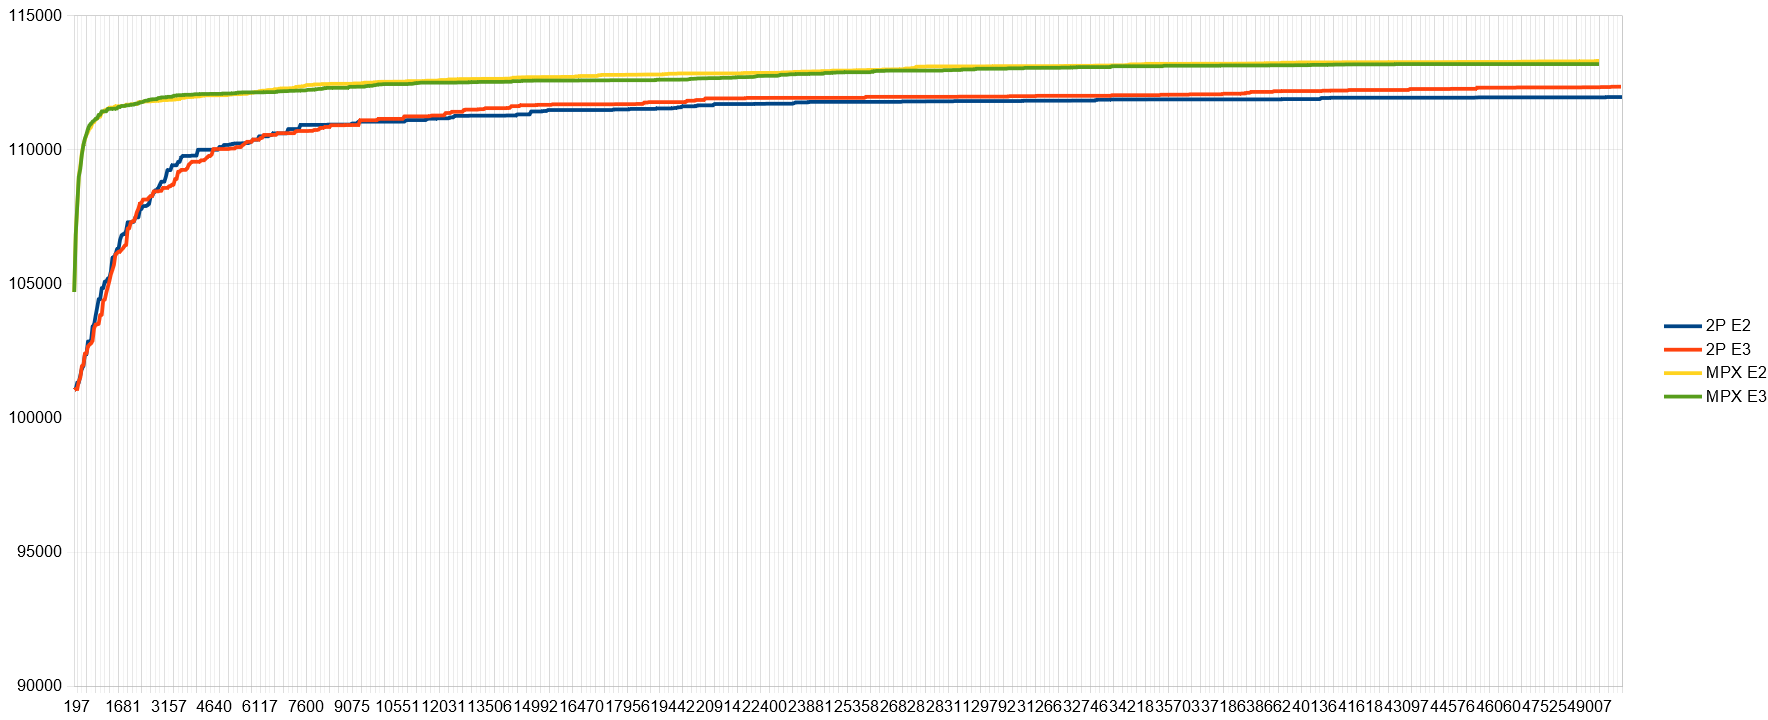
\includegraphics[scale=0.3]{img/35608477_MDG-a_21_n2000_m200.png}
		\caption{Evolución del mejor coste en la ejecución de todos los algoritmos respecto al número de evaluaciones para el problema MDG-a21, semilla 35608477}
		\label{MDG-a_21_historico}
	\end{figure}

	\paragraph{}Para el problema MDG-a21 los algoritmos MPX empiezan a encontrar soluciones aceptables en torno a las 100 evaluaciones realizadas para los dos elitismos. Los algoritmos de cruce en dos puntos empiezan a obtener soluciones aceptables a partir de las 545 evaluaciones para una élite = 2, y a partir de las 692 evaluaciones para una élite = 3. En este problema las soluciones óptimas son todas aquellas cuyo coste es superior a 102.833,1.
	
	\paragraph{}En la ejecución del algoritmo MPX con un elitismo = 2, no se estabiliza el mejor coste en un valor fijo, sino que se va mejorando continuamente, llegando a obtener el coste final obtenido = 113.312 al llegar a las 49.900 evaluaciones realizadas.
	
	\paragraph{}En la ejecución del algoritmo MPX con un elitismo = 3, el mejor coste obtenido se estabiliza en 113.193 a partir de las 43.350 evaluaciones, permaneciendo inalterable hasta alcanzar las 50.000 evaluaciones objetivo.
	
	\paragraph{}En la ejecución del algoritmo de corte en dos puntos con un elitismo = 2, no se estabiliza el mejor coste en un valor fijo, sino que se va mejorando continuamente, llegando a obtener el coste final obtenido = 111.963 al llegar a las 49.554 evaluaciones realizadas.
	
	\paragraph{}En la ejecución del algoritmo de corte en dos puntos con un elitismo = 3, no se estabiliza el mejor coste en un valor fijo, sino que se va mejorando continuamente, llegando a obtener el coste final obtenido = 112.350 al llegar a las 49.926 evaluaciones realizadas.
	
	\paragraph{}En el algoritmo MPX con un elitismo = 2 obtenemos un coste final = 113.312, que difiere del óptimo global en un 0,008\% aproximadamente. El óptimo global para este problema es 114.259.
	
	\paragraph{}En el algoritmo MPX con un elitismo = 3 obtenemos un coste final = 113.193, que difiere del óptimo global en un 0,009\% aproximadamente.
	
	\paragraph{}En el algoritmo de corte en dos puntos con un elitismo = 2 obtenemos un coste final = 111.963, que difiere del óptimo global en un 0,02\% aproximadamente.
	
	\paragraph{}En el algoritmo de corte en dos puntos con un elitismo = 3 obtenemos un coste final = 112.350, que difiere del óptimo global en un 0,02\% aproximadamente.
	
	\begin{figure}[H]
		\centering
		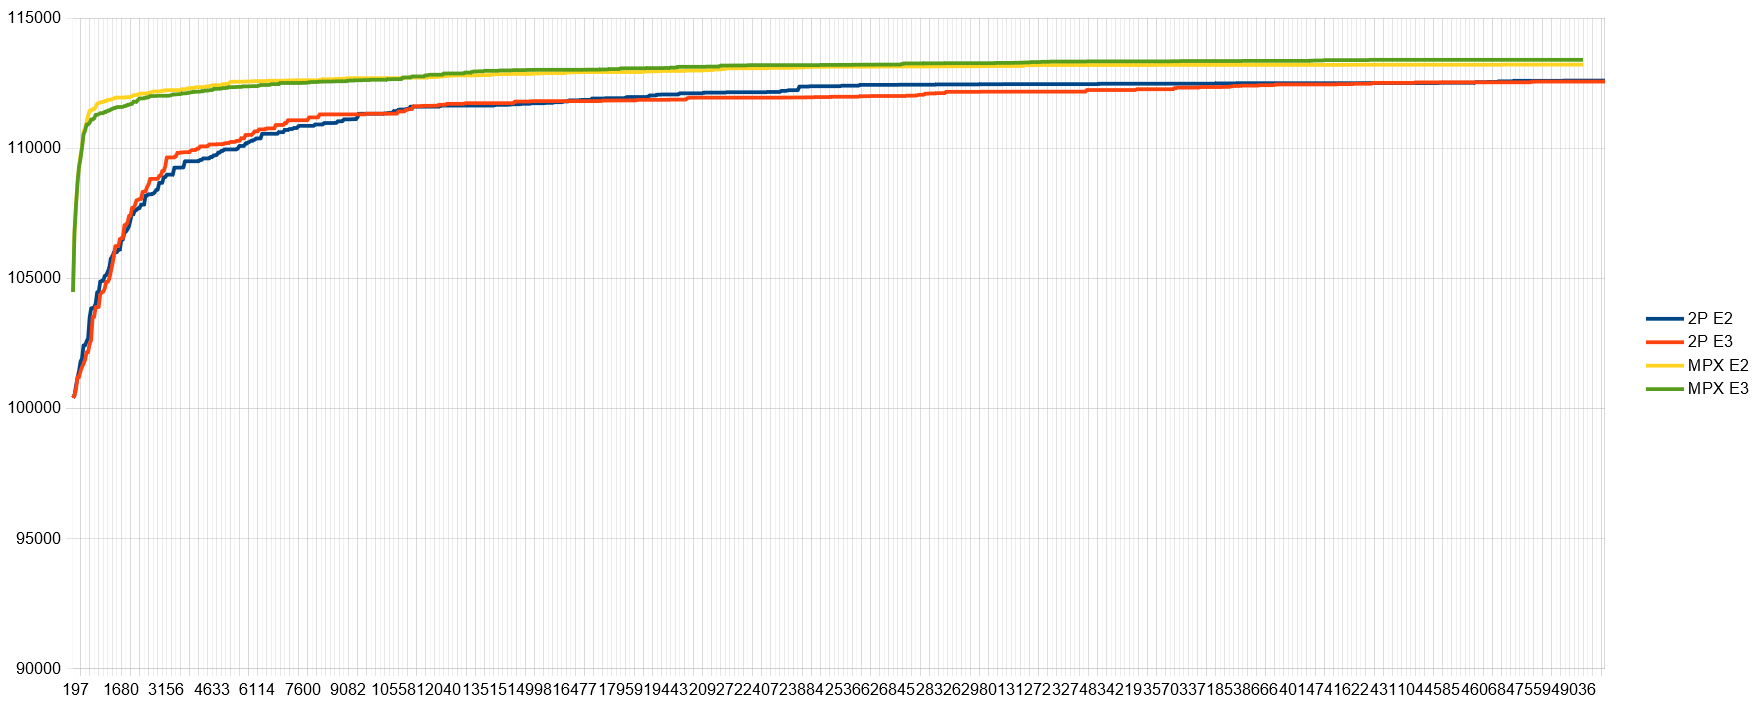
\includegraphics[scale=0.3]{img/35608477_MDG-a_22_n2000_m200.png}
		\caption{Evolución del mejor coste en la ejecución de todos los algoritmos respecto al número de evaluaciones para el problema MDG-a22, semilla 35608477}
		\label{MDG-a_22_historico}
	\end{figure}

	\paragraph{}Para el problema MDG-a22 los algoritmos MPX empiezan a encontrar soluciones aceptables en torno a las 100 evaluaciones realizadas para los dos elitismos. Los algoritmos de cruce en dos puntos empiezan a obtener soluciones aceptables a partir de las 642 evaluaciones para una élite = 2, y a partir de las 738 evaluaciones para una élite = 3. En este problema las soluciones óptimas son todas aquellas cuyo coste es superior a 102.894,3.
	
	\paragraph{}En la ejecución del algoritmo MPX con un elitismo = 2, no se estabiliza el mejor coste en un valor fijo, sino que se va mejorando continuamente, llegando a obtener el coste final obtenido = 113.217 al llegar a las 47.350 evaluaciones realizadas.
	
	\paragraph{}En la ejecución del algoritmo MPX con un elitismo = 3, no se estabiliza el mejor coste en un valor fijo, sino que se va mejorando continuamente, llegando a obtener el coste final obtenido = 113.402 al llegar a las 42.950 evaluaciones realizadas.

	\paragraph{}En la ejecución del algoritmo de corte en dos puntos con un elitismo = 2, no se estabiliza el mejor coste en un valor fijo, sino que se va mejorando continuamente, llegando a obtener el coste final obtenido = 112.604 al llegar a las 48.692 evaluaciones realizadas.
	
	\paragraph{}En la ejecución del algoritmo de corte en dos puntos con un elitismo = 3, no se estabiliza el mejor coste en un valor fijo, sino que se va mejorando continuamente, llegando a obtener el coste final obtenido = 112.564 al llegar a las 47.679 evaluaciones realizadas.
	
	\paragraph{}En el algoritmo MPX con un elitismo = 2 obtenemos un coste final = 113.217, que difiere del óptimo global en un 0,01\% aproximadamente. El óptimo global para este problema es 114.327.
	
	\paragraph{}En el algoritmo MPX con un elitismo = 3 obtenemos un coste final = 113.402, que difiere del óptimo global en un 0,009\% aproximadamente.
	
	\paragraph{}En el algoritmo de corte en dos puntos con un elitismo = 2 obtenemos un coste final = 112.604, que difiere del óptimo global en un 0,02\% aproximadamente.
	
	\paragraph{}En el algoritmo de corte en dos puntos con un elitismo = 3 obtenemos un coste final = 112.564, que difiere del óptimo global en un 0,02\% aproximadamente.

	\begin{figure}[H]
		\centering
		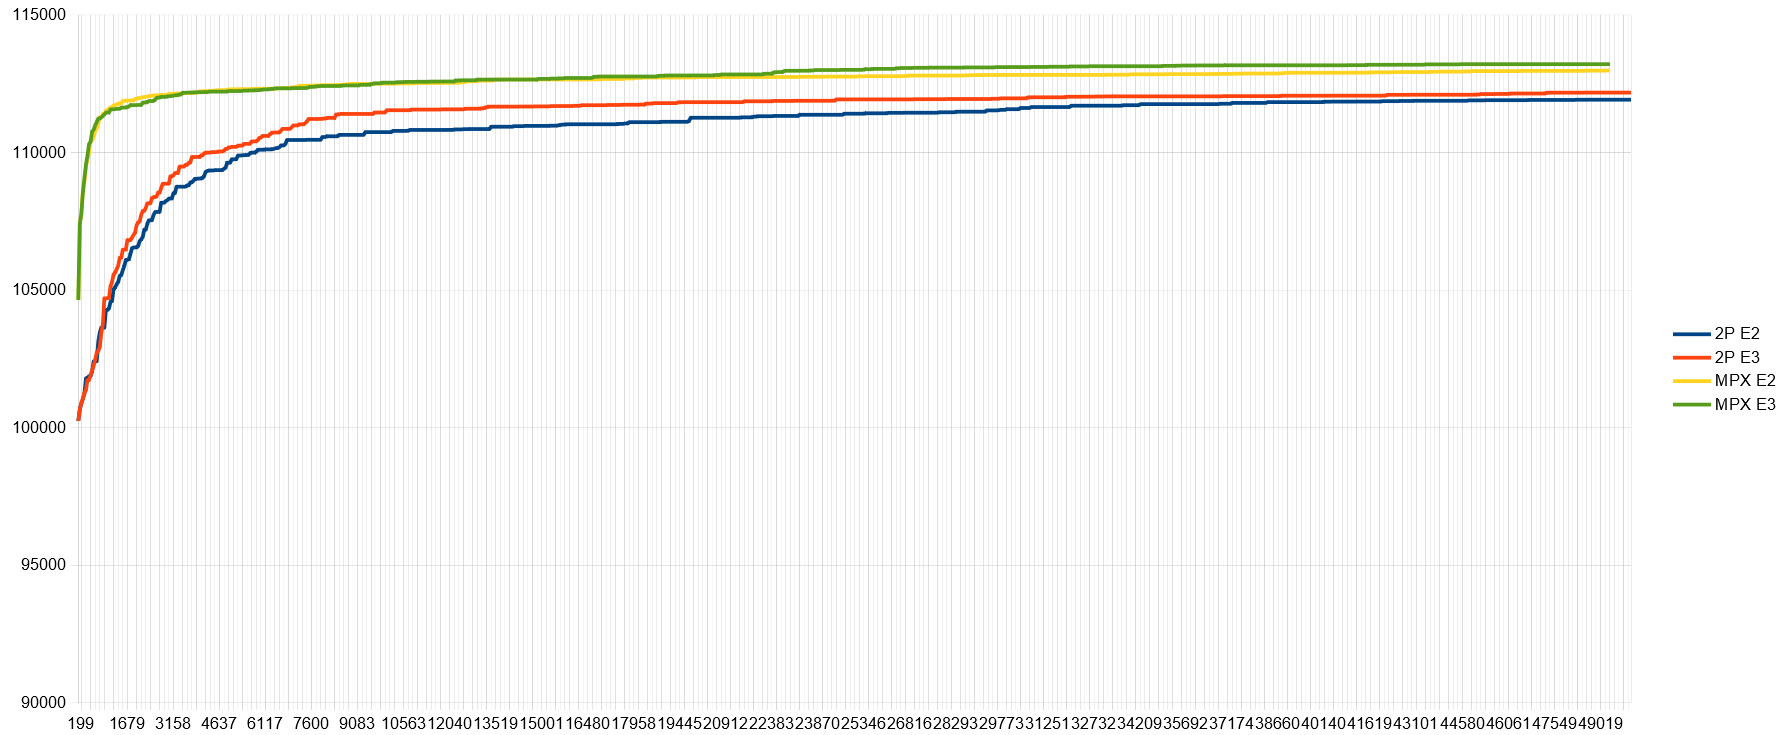
\includegraphics[scale=0.3]{img/35608477_MDG-a_23_n2000_m200.png}
		\caption{Evolución del mejor coste en la ejecución de todos los algoritmos respecto al número de evaluaciones para el problema MDG-a23, semilla 35608477}
		\label{MDG-a_23_historico}
	\end{figure}

	\paragraph{}Para el problema MDG-a22 los algoritmos MPX empiezan a encontrar soluciones aceptables en torno a las 100 evaluaciones realizadas para los dos elitismos. Los algoritmos de cruce en dos puntos empiezan a obtener soluciones aceptables a partir de las 741 evaluaciones para una élite = 2, y a partir de las 692 evaluaciones para una élite = 3. En este problema las soluciones óptimas son todas aquellas cuyo coste es superior a 102.710,7.
	
	\paragraph{}En la ejecución del algoritmo MPX con un elitismo = 2, no se estabiliza el mejor coste en un valor fijo, sino que se va mejorando continuamente, llegando a obtener el coste final obtenido = 112.982 al llegar a las 49.900 evaluaciones realizadas.
	
	\paragraph{}En la ejecución del algoritmo MPX con un elitismo = 3, no se estabiliza el mejor coste en un valor fijo, sino que se va mejorando continuamente, llegando a obtener el coste final obtenido = 113.212 al llegar a las 45.150 evaluaciones realizadas.
	
	\paragraph{}En la ejecución del algoritmo de corte en dos puntos con un elitismo = 2, no se estabiliza el mejor coste en un valor fijo, sino que se va mejorando continuamente, llegando a obtener el coste final obtenido = 111.921 al llegar a las 48.627 evaluaciones realizadas.
	
	\paragraph{}En la ejecución del algoritmo de corte en dos puntos con un elitismo = 3, no se estabiliza el mejor coste en un valor fijo, sino que se va mejorando continuamente, llegando a obtener el coste final obtenido = 112.178 al llegar a las 48.561 evaluaciones realizadas.
	
	\paragraph{}En el algoritmo MPX con un elitismo = 2 obtenemos un coste final = 112.982, que difiere del óptimo global en un 0,01\% aproximadamente. El óptimo global para este problema es 114.123.
	
	\paragraph{}En el algoritmo MPX con un elitismo = 3 obtenemos un coste final = 113.212, que difiere del óptimo global en un 0,008\% aproximadamente.
	
	\paragraph{}En el algoritmo de corte en dos puntos con un elitismo = 2 obtenemos un coste final = 111.921, que difiere del óptimo global en un 0,02\% aproximadamente.
	
	\paragraph{}En el algoritmo de corte en dos puntos con un elitismo = 3 obtenemos un coste final = 112.178, que difiere del óptimo global en un 0,02\% aproximadamente.
			
	
	\subsubsection{Cruce MPX con elitismo 2 vs elitismo 3}
	
		\begin{table}[H]
		\begin{center}
			\begin{tabular}{| c | c | c | c | c | c | c |}
				\hline
				\multicolumn{7}{ |c| }{Genético MPX elite 2} \\ \hline
				 & \multicolumn{2}{ |c| }{GKD-c\_1\_n500\_m50} & \multicolumn{2}{ |c| }{GKD-c\_2\_n500\_m50} & \multicolumn{2}{ |c| }{GKD-c\_3\_n500\_m50} \\ \hline
				Ejecución & Coste & Tiempo & Coste & Tiempo & Coste & Tiempo \\ \hline
				1 & 19481,688 & 892,00 & 19700,36 & 892,00 & 19547,215 & 888,00 \\
				2 &19481,69 & 909,00 & 19700,36 & 897,00 & 19547,22 & 893,00\\
				3 &19485,19	& 918,00 & 19700,34	& 886,00 & 19547,22	& 894,00\\
				4 &19480,68 & 895,00 & 19699,48	& 1731,00 & 19543,93 & 895,00\\
				5 &19485,19	& 901,00 & 19700,88	& 905,00 & 19547,22	& 890,00\\ \hline
				Media &-0,01\% & 903 & -0,01\%	& 1062 & 0,00\%	& 892,00\\ \hline
				Desviación Típica  & 0,01\%	& 10,61 & 0,00\% & 373,94 & 0,01\% & 2,92\\ \hline
			\end{tabular}
			\caption{Resultados GKD}
			\label{tab:tabMPXE2GKD}
		\end{center}
	\end{table} 


	\begin{table}[H]
		\begin{center}
			\begin{tabular}{| c | c | c | c | c | c | c |}
				\hline
				\multicolumn{7}{ |c| }{Genético MPX elite 2} \\ \hline
				& \multicolumn{2}{ |c| }{SOM-b\_11\_n300\_m90} & \multicolumn{2}{ |c| }{SOM-b\_12\_n300\_m120} & \multicolumn{2}{ |c| }{SOM-b\_13\_n400\_m40} \\ \hline
				Ejecución & Coste & Tiempo & Coste & Tiempo & Coste & Tiempo\\\hline
				1 &20708,00	&2288,00 & 35866,00	& 4717,00 & 4619,00 & 597,00\\
				2 &20727,00	& 2404,00 & 35847,00 & 4535,00 & 4581,00 & 616,00\\
				3 &20651,00	& 2407,00 & 35871,00 & 4746,00 & 4595,00 & 604,00\\
				4 &20650,00	& 2260,00 & 35872,00 & 4546,00 & 4534,00 & 599,00\\
				5 &20713,00	& 2299,00 & 35844,00 & 4800,00 & 4570,00 &606,00\\\hline
				Media &-0,26\% & 2331,60 & -0,06\% & 4668,80 & -1,68\% & 604,40\\ \hline
				Desviación Típica  & 0,18\%	& 68,95 & 0,04\% & 120,91 & 0,68\%	& 7,44 \\ \hline
			\end{tabular}
			\caption{Resultados SOM}
			\label{tab:tabMPXE2SOM}
		\end{center}
	\end{table} 

	\begin{table}[H]
		\begin{center}
			\begin{tabular}{| c | c | c | c | c | c | c |}
				\hline
				\multicolumn{7}{ |c| }{Genético MPX elite 2} \\ \hline
				& \multicolumn{2}{ |c| }{MDG-a\_21\_n2000\_m200} & \multicolumn{2}{ |c| }{MDG-a\_22\_n2000\_m200} & \multicolumn{2}{ |c| }{MDG-a\_23\_n2000\_m200}\\\hline
				Ejecución & Coste & Tiempo & Coste & Tiempo & Coste & Tiempo\\\hline
				1 &113460,00 & 30888,00	& 112852,00	& 29847,00 & 112933,00 & 29246,00\\
				2 &113135,00 & 28109,00	& 112957,00	& 28412,00 & 113487,00 & 28296,00\\
				3 &113312,00 & 28749,00	& 113217,00	& 28307,00 & 112982,00 & 29794,00\\
				4 &113112,00 & 27848,00	& 113059,00	& 29327,00 & 113251,00 & 29338,00\\
				5 &113088,00 & 28269,00	& 112829,00	&28468,00 & 112789,00 & 30736,00\\\hline
				Media &-0,91\% & 28772,60 & -1,18\% & 28872,20 & -0,91 & 29482,00\\ \hline
				Desviación Típica & 0,14\%	& 1227,23 & 0,14\% & 680,38 & 0,24\% & 887,82 \\ \hline
			\end{tabular}
			\caption{Resultados MDG}
			\label{tab:tabMPXE2MDG}
		\end{center}
	\end{table}

	\begin{table}[H]
		\begin{center}
			\begin{tabular}{| c | c | c | c | c | c | c |}
				\hline
				\multicolumn{7}{ |c| }{Genético MPX elite 3} \\ \hline
				& \multicolumn{2}{ |c| }{GKD-c\_1\_n500\_m50} & \multicolumn{2}{ |c| }{GKD-c\_2\_n500\_m50} & \multicolumn{2}{ |c| }{GKD-c\_3\_n500\_m50} \\ \hline
				Ejecución & Coste & Tiempo & Coste & Tiempo & Coste & Tiempo \\ \hline
				1 &19481,69 &874,00	& 19701,52 & 884,00 & 19547,22 & 882,00\\
				2 &19482,37 & 872,00 & 19701,52 & 888,00 & 19547,22 & 1354,00\\
				3 &19485,19 & 892,00 & 19701,52 & 877,00 & 19547,22 & 892,00\\
				4 &19485,19 & 879,00 & 19699,48 & 883,00 & 19547,22 & 890,00\\
				5 &19485,19 & 875,00 & 19701,52 & 873,00 & 19543,48 & 881,00\\ \hline
				Media &0,00\% & 1173,40 & 0,00\% & 1118,60 & 0,00\% & 979,80\\ \hline
				Desviación Típica & 0,01\%	& 8,02 & 0,00\% & 5,96 & 0,01\% & 209,24 \\ \hline
			\end{tabular}
			\caption{Resultados GKD}
			\label{tab:tabMPXE3GKD}
		\end{center}
	\end{table} 


	\begin{table}[H]
		\begin{center}
			\begin{tabular}{| c | c | c | c | c | c | c |}
				\hline
				\multicolumn{7}{ |c| }{Genético MPX elite 3} \\ \hline
				& \multicolumn{2}{ |c| }{SOM-b\_11\_n300\_m90} & \multicolumn{2}{ |c| }{SOM-b\_12\_n300\_m120} & \multicolumn{2}{ |c| }{SOM-b\_13\_n400\_m40} \\ \hline
				Ejecución & Coste & Tiempo & Coste & Tiempo & Coste & Tiempo\\\hline
				1 &20648,00 & 2252,00 & 35870,00 & 4404,00 & 4590,00 & 1219,00\\
				2 &20731,00	& 2253,00 & 35866,00 & 4190,00 & 4625,00 & 612,00\\
				3 &20650,00	& 2128,00 & 35834,00 & 4424,00 & 4584,00 & 617,00\\
				4 &20672,00	& 2238,00 & 35879,00 & 4272,00 & 4553,00 & 602,00\\
				5 &20647,00 & 2215,00 & 35825,00 & 5704,00 & 4578,00 & 602,00\\\hline
				Media &-0,35\% & 2217,20 & -0,07\% & 4598,80 & -1,55\% & 730,40\\ \hline
				Desviación Típica & 0,17\%	& 52,17 & 0,07\% & 625,28 & 0,56\% & 273,21 \\ \hline
			\end{tabular}
			\caption{Resultados SOM}
			\label{tab:tabMPXE3SOM}
		\end{center}
	\end{table} 

	\begin{table}[H]
		\begin{center}
			\begin{tabular}{| c | c | c | c | c | c | c |}
				\hline
				\multicolumn{7}{ |c| }{Genético MPX elite 3} \\ \hline
				& \multicolumn{2}{ |c| }{MDG-a\_21\_n2000\_m200} & \multicolumn{2}{ |c| }{MDG-a\_22\_n2000\_m200} & \multicolumn{2}{ |c| }{MDG-a\_23\_n2000\_m200}\\\hline
				Ejecución & Coste & Tiempo & Coste & Tiempo & Coste & Tiempo\\\hline
				1 &112931,00 & 28983,00 & 113173,00 & 27009,00 & 112978,00 & 27013,00\\
				2 &113375,00 & 28527,00	& 113335,00	& 26306,00 & 113350,00 & 26662,00\\
				3 &113193,00 & 27110,00 & 113402,00 & 27403,00 & 113212,00 & 26661,00\\
				4 &113074,00 & 28232,00	& 112677,00	& 24702,00 & 113274,00 & 25797,00\\
				5 &113445,00 & 26549,00	& 113470,00	& 27643,00 & 112600,00 & 26081,00\\\hline
				Media &-0,92\% & 27880,20 & -0,98\% & 26612,60 & -0,91\% & 26442,80\\ \hline
				Desviación Típica & 0,19\%	& 1015,33 & 0,28\% & 1181,95 & 0,27\% & 492,12 \\ \hline
			\end{tabular}
			\caption{Resultados MDG}
			\label{tab:tabMPXE3MDG}
		\end{center}
	\end{table}


	
	\paragraph{} El operador de cruce MPX aplicado a la serie de datos GKD, con una élite de 2 o 3 individuos, ofrece unos resultados muy similares respecto a coste.
	
	\paragraph{} Para el archivo GKD-c1  (\ref{gkd-c1_coste}), los resultados obtenidos en las diferentes iteraciones, son similares, ofreciendo un ligero mayor agrupamiento de los resultados a favor de la élite de 3 individuos.
	
	\paragraph{} Para el archivo GKD-c2  (\ref{gkd-c2_coste}),los resultados son ligeramente superiores con una élite de 3 individuos.
	
	\paragraph{} Para el archivo GKD-c3  (\ref{gkd-c3_coste}), los resultados revelan un comportamiento similar.
	
	
	\begin{figure}[H]
		
		\centering
		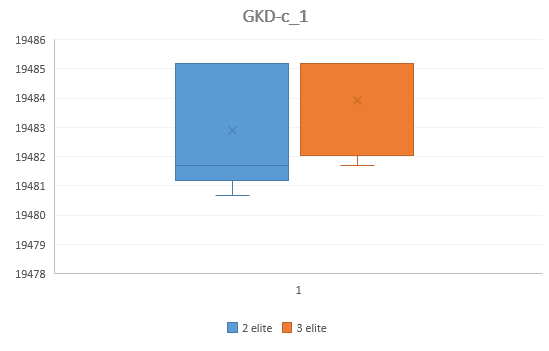
\includegraphics[scale=0.7]{img/MPX_2vs3/GKD-c_1_Costes}
		\caption{Costes obtenidos para el archivo GKD-c1, con una élite de 2 y 3}
		\label{gkd-c1_coste}
	\end{figure}
	\begin{figure}[H]
		\centering
		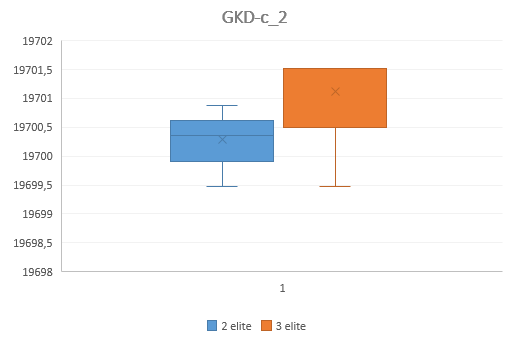
\includegraphics[scale=0.7]{img/MPX_2vs3/GKD-c_2_Costes}
		\caption{Costes obtenidos para el archivo GKD-c2, con una élite de 2 y 3}
		\label{gkd-c2_coste}
		
	\end{figure}
	\begin{figure}[H]
		\centering
		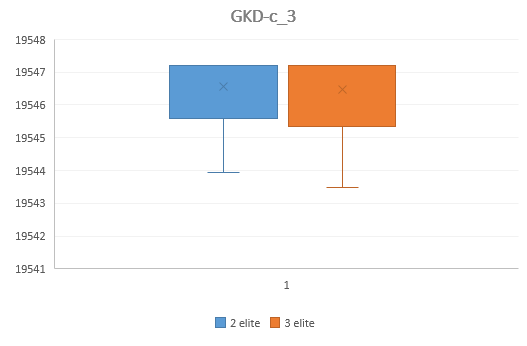
\includegraphics[scale=0.7]{img/MPX_2vs3/GKD-c_3_Costes}
		\caption{Costes obtenidos para el archivo GKD-c3, con una élite de 2 y 3}
		\label{gkd-c3_coste}
		
		
	\end{figure}

		\paragraph{} El operador de cruce MPX aplicado a la serie de datos SOM, con una élite de 2 o 3 individuos, ofrece unos resultados muy similares respecto a coste.

	\begin{figure}[H]
		
		\centering
		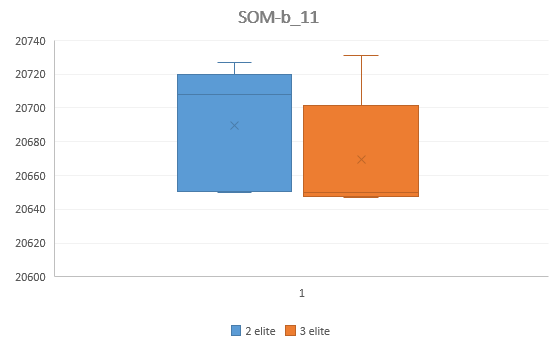
\includegraphics[scale=0.7]{img/MPX_2vs3/SOM-b_11_Costes}
		\caption{Costes obtenidos para el archivo SOM-b11, con una élite de 2 y 3}
		\label{som-b11_coste}
		
	\end{figure}
	\begin{figure}[H]
		\centering
		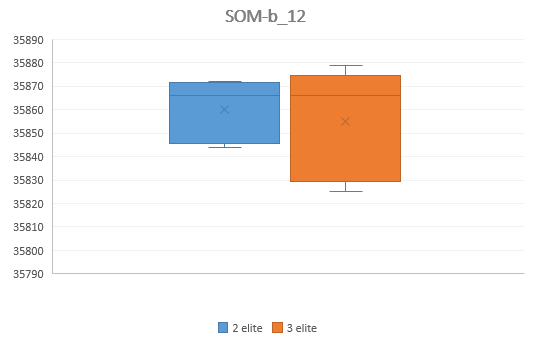
\includegraphics[scale=0.7]{img/MPX_2vs3/SOM-b_12_Costes}
		\caption{Costes obtenidos para el archivo SOM-b12, con una élite de 2 y 3}
		\label{som-b12_coste}
		
	\end{figure}
	\begin{figure}[H]
		\centering
		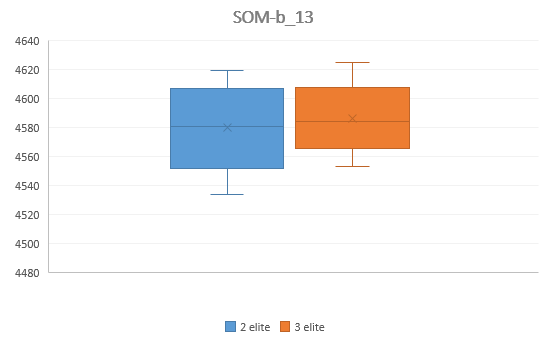
\includegraphics[scale=0.7]{img/MPX_2vs3/SOM-b_13_Costes}
		\caption{Costes obtenidos para el archivo SOM-b13, con una élite de 2 y 3}
		\label{som-b13_coste}
		
		
	\end{figure}


	\subsubsection{Cruce en dos puntos con elitismo 2 vs elitismo 3}
	
	\paragraph{}De la experimentación realizada, obtenemos los siguientes datos
	
	\begin{table}[H]
		\begin{center}
			\begin{tabular}{| c | c | c | c | c | c | c |}
				\hline
				\multicolumn{7}{ |c| }{Genético 2 puntos elite 2} \\ \hline
				& \multicolumn{2}{ |c| }{GKD-c\_1\_n500\_m50} & \multicolumn{2}{ |c| }{GKD-c\_2\_n500\_m50} & \multicolumn{2}{ |c| }{GKD-c\_3\_n500\_m50} \\ \hline
				Ejecución & Coste & Tiempo & Coste & Tiempo & Coste & Tiempo \\ \hline
				1 &19485,19 & 1205,00 & 19700,36 & 1131,00 & 19547,22 & 1169,00\\
				2 &19485,19 & 1184,00 & 19701,52 & 1109,00 & 19547,22 & 1121,00\\
				3 &19485,19	& 1142,00 & 19701,52 & 1118,00 & 19547,22 & 1109,00\\
				4 &19485,19	& 1179,00 & 19701,52 & 1103,00 & 19547,22 & 1112,00\\
				5 &19485,19 & 1157,00 & 19700,36 & 1132,00 & 19547,22 & 1121,00\\ \hline
				Media & 0,00\% & 1173,40 & 0,00\% & 1118,60 & 0,00\% & 1126,40\\ \hline
				Desviación Típica & 0,00\%	& 24,48 & 0,00\% & 12,93 & 0,00\% & 24,41 \\ \hline
			\end{tabular}
			\caption{Resultados GKD}
			\label{tab:tab2POINTE2GKD}
		\end{center}
	\end{table} 
	
	
	\begin{table}[H]
		\begin{center}
			\begin{tabular}{| c | c | c | c | c | c | c |}
				\hline
				\multicolumn{7}{ |c| }{Genético 2 puntos elite 2} \\ \hline
				& \multicolumn{2}{ |c| }{SOM-b\_11\_n300\_m90} & \multicolumn{2}{ |c| }{SOM-b\_12\_n300\_m120} & \multicolumn{2}{ |c| }{SOM-b\_13\_n400\_m40} \\ \hline
				Ejecución & Coste & Tiempo & Coste & Tiempo & Coste & Tiempo\\\hline
				1 &20644,00 & 1807,00 & 35848,00 & 3839,00 & 4631,00 & 1211,00\\
				2 &20650,00	& 1752,00 & 35813,00 & 3751,00 & 4542,00 & 1054,00\\
				3 &20631,00	& 1786,00 & 35847,00 & 3449,00 & 4571,00 & 817,00\\
				4 &20674,00	& 1825,00 & 35803,00 & 3713,00 & 4614,00 & 646,00\\
				5 &20638,00 & 1800,00 & 35871,00 & 3847,00 & 4540,00 & 657,00\\\hline
				Media &-0,46\% & 1794,00 & -0,12\% & 3719,80 & -1,68\% & 877,00\\ \hline
				Desviación Típica & 0,08\%	& 27,36 & 0,08\% & 161,82 & 0,89\% & 249,12 \\ \hline
			\end{tabular}
			\caption{Resultados SOM}
			\label{tab:tab2POINTE2SOM}
		\end{center}
	\end{table} 
	
	\begin{table}[H]
		\begin{center}
			\begin{tabular}{| c | c | c | c | c | c | c |}
				\hline
				\multicolumn{7}{ |c| }{Genético 2 puntos elite 2} \\ \hline
				& \multicolumn{2}{ |c| }{MDG-a\_21\_n2000\_m200} & \multicolumn{2}{ |c| }{MDG-a\_22\_n2000\_m200} & \multicolumn{2}{ |c| }{MDG-a\_23\_n2000\_m200}\\\hline
				Ejecución & Coste & Tiempo & Coste & Tiempo & Coste & Tiempo\\\hline
				1 &112242,00 & 44907,00 & 112506,00 & 46008,00 & 111991,00 & 44417,00\\
				2 &112280,00 & 43616,00 & 112443,00	& 43669,00 & 112497,00 & 43752,00\\
				3 &111963,00 & 45431,00	& 112604,00	& 44006,00 & 111921,00 & 44011,00\\
				4 &112012,00 & 42691,00	& 112723,00	& 43679,00 & 112302,00 & 43656,00\\
				5 &112367,00 & 44207,00	& 111886,00	& 43836,00 & 112163,00 & 43111,00\\\hline
				Media &-1,83\% & 44170,40 & -1,66\% & 44239,60 & -1,71\% & 43789,40\\ \hline
				Desviación Típica & 0,15\%	& 1075,76 & 0,28\% & 998,07 & 0,20\% & 480,21 \\ \hline
			\end{tabular}
			\caption{Resultados MDG}
			\label{tab:tab2POINTE2MDG}
		\end{center}
	\end{table}
	
	\begin{table}[H]
		\begin{center}
			\begin{tabular}{| c | c | c | c | c | c | c |}
				\hline
				\multicolumn{7}{ |c| }{Genético 2 puntos elite 3} \\ \hline
				& \multicolumn{2}{ |c| }{GKD-c\_1\_n500\_m50} & \multicolumn{2}{ |c| }{GKD-c\_2\_n500\_m50} & \multicolumn{2}{ |c| }{GKD-c\_3\_n500\_m50} \\ \hline
				Ejecución & Coste & Tiempo & Coste & Tiempo & Coste & Tiempo \\ \hline
				1 &19485,19	& 1081,00 & 19701,52 & 1048,00 & 19547,22 & 1049,00\\
				2 &19485,19	& 1080,00 & 19700,36 & 1037,00 & 19547,22 & 1079,00\\
				3 &19485,19	& 1054,00 & 19701,52 & 1012,00 & 19547,22 & 1069,00\\
				4 &19485,19	& 1085,00 & 19701,52 & 1030,00 & 19547,22 & 2404,00\\
				5 &19485,19	& 1061,00 & 19701,52 & 1038,00 & 19547,22 & 1079,00\\ \hline
				Media &0,00\% & 1172,20 & 0,00\% & 1033,00 & 0,00\% & 1336,00\\ \hline
				Desviación Típica & 0,00\%	& 13,77 & 0,00\% & 13,38 & 0,00\% & 597,16 \\ \hline
			\end{tabular}
			\caption{Resultados GKD}
			\label{tab:tab2POINTE3GKD}
		\end{center}
	\end{table} 
	
	
	\begin{table}[H]
		\begin{center}
			\begin{tabular}{| c | c | c | c | c | c | c |}
				\hline
				\multicolumn{7}{ |c| }{Genético 2 puntos elite 3} \\ \hline
				& \multicolumn{2}{ |c| }{SOM-b\_11\_n300\_m90} & \multicolumn{2}{ |c| }{SOM-b\_12\_n300\_m120} & \multicolumn{2}{ |c| }{SOM-b\_13\_n400\_m40} \\ \hline
				Ejecución & Coste & Tiempo & Coste & Tiempo & Coste & Tiempo\\\hline
				1 &20636,00	& 1744,00 & 35801,00 & 2501,00 & 4588,00 & 632,00\\
				2 &20666,00	& 1660,00 & 35863,00 & 2520,00 & 4572,00 & 595,00\\
				3 &20623,00	& 1658,00 & 35863,00 & 3165,00 & 4560,00 & 587,00\\
				4 &20662,00	& 1720,00 & 35860,00 & 2531,00 & 4646,00 & 608,00\\
				5 &20689,00	& 1701,00 & 35863,00 & 2540,00 & 4573,00 & 588,00\\\hline
				Media &-0,42\% & 1696,60 & -0,09\% & 2651,40 & -1,51\% & 602,00\\ \hline
				Desviación Típica & 0,13\%	& 37,56 & 0,08\% & 287,48 & 0,73\% & 18,75 \\ \hline
			\end{tabular}
			\caption{Resultados SOM}
			\label{tab:tab2POINTE3SOM}
		\end{center}
	\end{table} 
	
	\begin{table}[H]
		\begin{center}
			\begin{tabular}{| c | c | c | c | c | c | c |}
				\hline
				\multicolumn{7}{ |c| }{Genético 2 puntos elite 3} \\ \hline
				& \multicolumn{2}{ |c| }{MDG-a\_21\_n2000\_m200} & \multicolumn{2}{ |c| }{MDG-a\_22\_n2000\_m200} & \multicolumn{2}{ |c| }{MDG-a\_23\_n2000\_m200}\\\hline
				Ejecución & Coste & Tiempo & Coste & Tiempo & Coste & Tiempo\\\hline
				1 &112586,00 & 44120,00	& 112506,00	& 44754,00 & 112402,00 & 41142,00\\
				2 &112538,00 & 43647,00	& 112210,00	& 44155,00 & 112253,00 & 40152,00\\
				3 &112350,00 & 42045,00	& 112564,00	& 43279,00 & 112178,00 & 40173,00\\
				4 &112488,00 & 41706,00	& 112444,00	& 43776,00 & 112437,00 & 40842,00\\
				5 &112420,00 & 42935,00	& 112352,00	& 42549,00 & 112500,00 & 40781,00\\\hline
				Media &-1,56\% & 42890.60\% & -1,67\% & 43702,60 & -1,55\% & 40618,00\\ \hline
				Desviación Típica & 0,08\%	& 1025,17 & 0,12\% & 840,49 & 0,12\% & 437,75 \\ \hline
			\end{tabular}
			\caption{Resultados MDG}
			\label{tab:tab2POINTE3MDG}
		\end{center}
	\end{table}
	
	\paragraph{}
	
	
	
	\subsubsection{Cruce Mpx con elitismo 3 vs dos puntos con elitismo 3}
	
	\begin{table}[H]
		\begin{center}
			\begin{tabular}{| c | c | c | c | c | c | c |}
				\hline
				\multicolumn{7}{ |c| }{Tabla final} \\ \hline
				& \multicolumn{2}{ |c| }{GKD-c\_1\_n500\_m50} & \multicolumn{2}{ |c| }{GKD-c\_2\_n500\_m50} & \multicolumn{2}{ |c| }{GKD-c\_3\_n500\_m50} \\ \hline
				MPX, 2 Elite &-0,01\% & 903,00 & -0,01\% & 1062,20 & 0,00\% & 892,00\\ \hline
				MPX, 3 Elite &-0,01\% & 878,40 & 0,00\% & 881,00 & 0,00\% & 979,80\\ \hline
				2 puntos, 2 Elite &0,00\% & 1173,40 & 0,00\% & 1118,60 & 0,00\% & 1126,40\\ \hline
				2 puntos, 3 Elite & 0,00\% & 1072,20\% & 0,00\% & 1033,00 & 0,00\% & 1336,00\\ \hline
			\end{tabular}
			\caption{Resultados GKD}
			\label{tab:tabvsGKD}
		\end{center}
	\end{table}
	
	\begin{table}[H]
		\begin{center}
			\begin{tabular}{| c | c | c | c | c | c | c |}
				\hline
				\multicolumn{7}{ |c| }{Tabla final} \\ \hline
				& \multicolumn{2}{ |c| }{SOM-b\_11\_n300\_m90} & \multicolumn{2}{ |c| }{SOM-b\_12\_n300\_m120} & \multicolumn{2}{ |c| }{SOM-b\_13\_n400\_m40} \\ \hline
				MPX, 2 Elite &-0,26\% & 2331,60 & -0,06\% & 4668,80 & -1,68 & 604,40\\ \hline
				MPX, 3 Elite &-0,35\% & 2217,20 & -0,07\% & 4598,80 & -1,55\% & 730,40\\ \hline
				2 puntos, 2 Elite &-0,46\% & 1794,00 & -0,12\% & 3719,80 & -1,68\% & 877,00\\ \hline
				2 puntos, 3 Elite &-0,42\% & 1696,60\% & -0,09\% & 2651,40 & -1,51\% & 602,00\\ \hline
			\end{tabular}
			\caption{Resultados SOM}
			\label{tab:tabvsSOM}
		\end{center}
	\end{table}
	
	\begin{table}[H]
		\begin{center}
			\begin{tabular}{| c | c | c | c | c | c | c |}
				\hline
				\multicolumn{7}{ |c| }{Tabla final} \\ \hline
				& \multicolumn{2}{ |c| }{MDG-a\_21\_n2000\_m200} & \multicolumn{2}{ |c| }{MDG-a\_22\_n2000\_m200} & \multicolumn{2}{ |c| }{MDG-a\_23\_n2000\_m200}\\\hline
				MPX, 2 Elite &-0,91\% & 28772,60 & -1,18\% & 28872,20 & -0,91 & 29482,00\\ \hline
				MPX, 3 Elite &-0,92\% & 27880,20 & -0,98\% & 26612,60 & -0,91\% & 26442,80\\ \hline
				2 puntos, 2 Elite &-1,83\% & 44170,40 & -1,66\% & 44239,60 & -1,71\% & 43789,40\\ \hline
				2 puntos, 3 Elite &-1,56\% & 42890.60\% & -1,67\% & 43702,60 & -1,55\% & 40618,00\\ \hline
			\end{tabular}
			\caption{Resultados MDG}
			\label{tab:tabvsMDG}
		\end{center}
	\end{table}
	
	\paragraph{} Si evaluamos los costes obtenidos, podemos observar que los dos operadores de cruce se comportan de manera similar en las instancias de datos GKD, no obstante, para el resto de datos, el cruce MPX ofrece unos resultados considerablemente mejores respecto al cruce en dos puntos, esto puede deberse a la estrategia de reparación de los cromosomas, la cuál, difiere entre un tipo de cruce y otro.
	
	\paragraph{}El cruce MPX genera más genes de los deseados, y para reparar los cromosomas, se emplea una estrategia de reparación basada en la eliminación de los genes que menos aportan al coste de la solución. Sin embargo, el cruce en dos puntos, genera menos genes de los deseados, y la estrategia empleada es la de incluir los genes que más aportan a la solución, que no están contenidos en la solución.
	
	\paragraph{}Si procedemos a evaluar la cantidad de tiempo empleada en obtener las soluciones, podemos observar que el cruce en dos puntos es hasta un 60\% más lento respecto al cruce mpx. La diferencia de tiempos, viene determinada por la estrategia de reparación de los cromosomas.
	
	\begin{figure}[H]
		\centering
		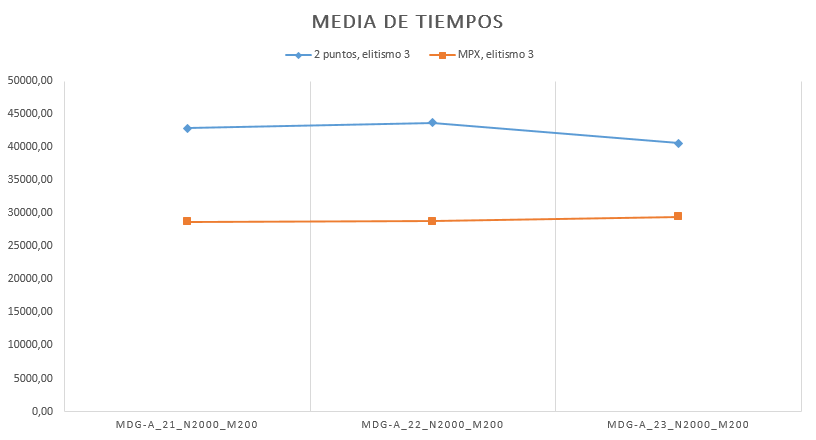
\includegraphics[scale=0.65]{img/MPXvs2Puntos/Tiempos}
		\caption{Media de tiempos para los distintos archivos MDG, tiempos expresados en milisegundos}
		\label{MDG_MPXvs2Puntos_Tiempos}
		
	\end{figure}
	
	\paragraph{}Como se ha indicado anteriormente, dicha estrategia difiere según el tipo de cruce. Para el cruce en dos puntos se necesita recorrer todos los elementos no seleccionados, e ir evaluando el coste que aportan, este proceso se repite hasta que los cromosomas tengan los genes necesarios, sin embargo, en el mpx solo necesitamos eliminar los genes del cromosoma que menos aportan. Por tanto, el número de operaciones necesarias es mayor en el caso del cruce en dos puntos.
	
	
	
	
	

	
	\paragraph{} 
	
